\chapter{Literature Review}
\label{chap:literature_review}

\section{Introduction}
Chatbot building tools have evolved from simple rule-based systems to AI-driven dynamic agents. However, most existing solutions focus either on static flow-based designs or fully AI-driven interactions, lacking a seamless integration of both approaches. This chapter reviews existing chatbot builders, automation platforms, and AI-driven chatbot frameworks to identify the gaps that FlowX aims to address.

\section{Theoretical Foundations}

\subsection{Rule-based Chatbots}

Rule-based chatbots follow predefined decision trees or workflows to respond to user input. These chatbots are deterministic and rely on explicit rules to generate responses. For example, a rule-based chatbot might ask a series of questions to gather information from the user and provide a specific response based on the answers. The next figure~\cite{medium_image} shows an example of a rule-based chatbot conversation flow diagram. It consists of a series of nodes representing decision points and transitions between them based on user input.
\begin{figure}[ht]
    \centering
    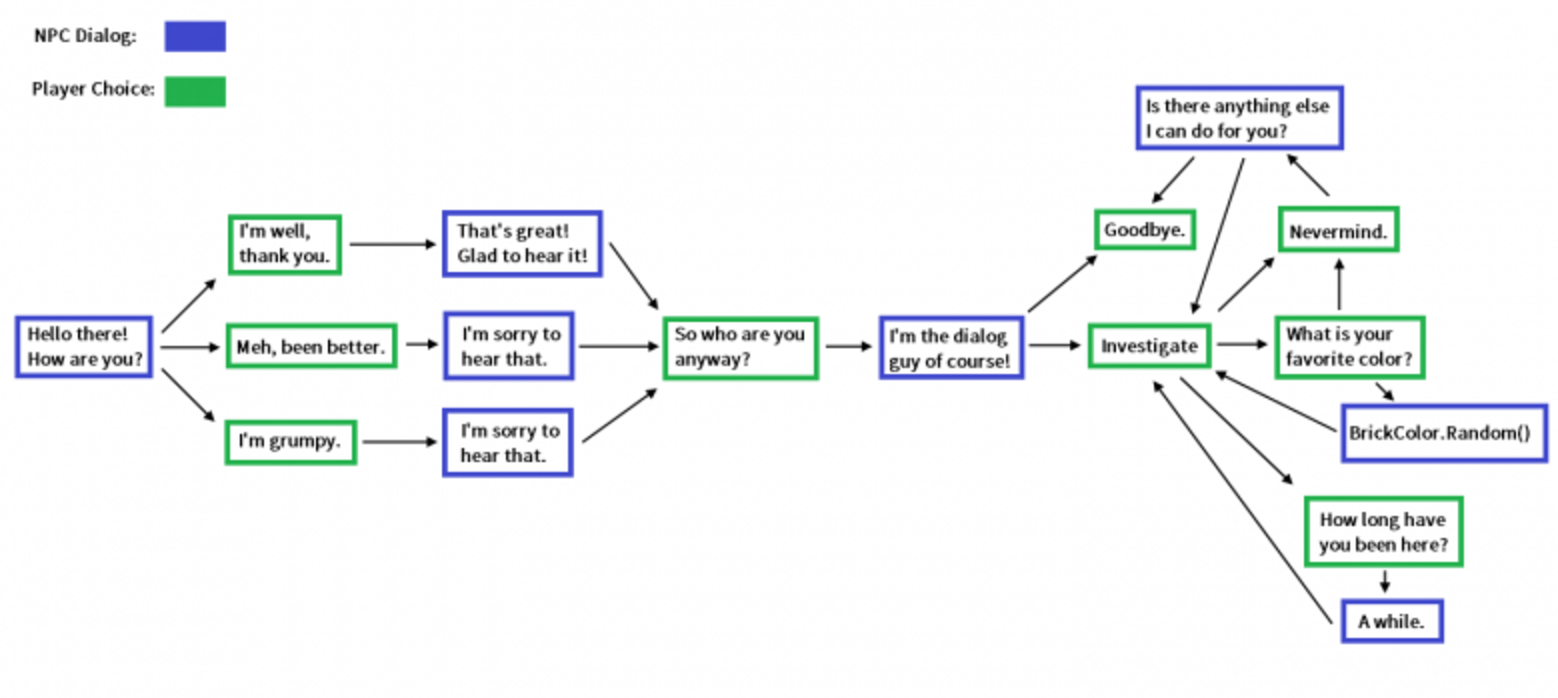
\includegraphics[width=0.7\textwidth]{assets/ChatbotConversationFlowExample.png}
    \caption{Example of a chatbot conversation flow diagram}
    \label{fig:chatbot_flow}
\end{figure}

\subsection{Generative Chatbots}

Generative chatbots leverage large language models (LLMs) like GPT-4 or Claude 3.5 Sonnet to produce contextually relevant responses. Unlike rule-based systems, these chatbots are probabilistic and generate outputs by learning patterns from training data, enabling flexible, open-ended interactions.

The next figure shows an example of a generative chatbot response generated by an LLM. In this example, the user input "explain how a combustion engine works" prompts the chatbot to generate a relevant response based on the context of the conversation.

\begin{figure}[ht]
    \centering
    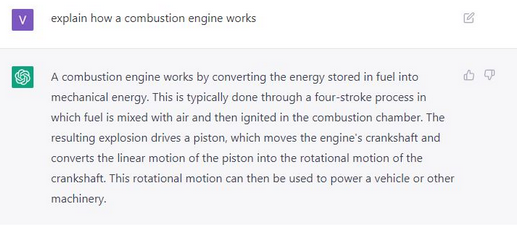
\includegraphics[width=0.7\textwidth]{assets/ChatgptMessageExample.png}
    \caption{Screenshot of a message from ChatGPT.}
    \label{fig:chatgpt_message}
\end{figure}

\subsection{Dynamic Routing}

Dynamic routing refers to the process where a system, such as a chatbot powered by a large language model (LLM), dynamically selects one of several predefined options or pathways based on the context of the user input. Instead of following a rigid, rule-based decision tree, the LLM evaluates the input and chooses the most appropriate response or action from a set of predefined choices. This allows for more flexible and context-aware interactions while still maintaining some level of control over the chatbot's behavior.

The next figure shows an example of dynamic routing in a chatbot conversation. The user gives a textual input, and the LLM evaluates it to determine what option to choose out of two possible responses. This gives the flow structure and more control over the conversation while still allowing for dynamic user interactions.

\begin{figure}[ht]
    \centering
    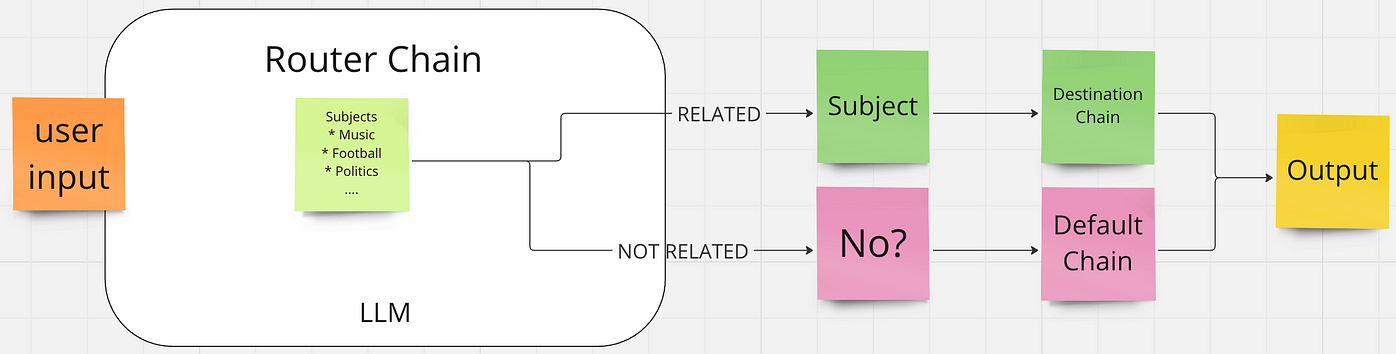
\includegraphics[width=0.8\textwidth]{assets/LangchainRouterChainExample.png}
    \caption{Example of dynamic routing in a chatbot conversation.}
    \label{fig:router_chain_example}
\end{figure}

\section{Existing Solutions and Their Approaches}

\subsection{No-Code Chatbot Builders}
No-code chatbot builders, such as Chatfuel~\cite{chatfuel}, Landbot~\cite{landbot}, and ManyChat~\cite{manychat}, allow users to create structured chatbot flows visually. These tools offer ease of use but are heavily reliant on predefined responses, which limits their adaptability to dynamic user input. For instance, they struggle to handle unexpected or unstructured queries, making them less suitable for complex conversational scenarios. While they excel in creating static, rule-based workflows, they lack the flexibility to adapt to more dynamic interactions. ManyChat, for example, is widely used for social media chatbots but is limited in its ability to handle complex, multi-turn conversations or integrate with advanced AI capabilities.

\subsection{Automation and Workflow Platforms}
Platforms like Zapier~\cite{zapier} and n8n~\cite{n8n} focus on workflow automation by connecting various services based on triggers and actions. While they excel in automating tasks, they do not offer built-in conversational capabilities or manage continuous user interactions. They can integrate with external tools, but they lack native support for multi-turn, context-aware conversations, limiting their use in chatbot development. These platforms are better suited for back-end automation rather than front-end conversational interfaces.

\subsection{NLP-Powered AI Chatbots}
Dialogflow~\cite{dialogflow} and Rasa~\cite{rasa} provide powerful NLP-driven chatbot solutions that utilize natural language processing (NLP) to understand user intent. These tools are highly adaptable and can handle dynamic user input, but often require significant technical expertise to set up and maintain. Furthermore, their reliance on AI and machine learning makes them unsuitable for users seeking simpler rule-based solutions. While they excel in handling unstructured conversations, they may be overkill and too advanced for simpler use cases.

\subsection{Hybrid Models}
Hybrid chatbot frameworks, such as Botpress~\cite{botpress} and Azure Bot Service~\cite{azurebot}, attempt to merge static workflows with dynamic adaptability. However, these solutions often require extensive manual setup and struggle to achieve a seamless balance between rule-based logic and dynamic interactions. For example, Botpress allows for custom scripting and integration with NLP models, but still prioritizes rule-based logic in many cases. Similarly, Azure Bot Service provides tools for integrating advanced capabilities, but the process can be complex and time-consuming, limiting its effectiveness for users who need simpler, more straightforward solutions.

\section{Identified Gaps in Existing Solutions}
The review of existing solutions reveals several key gaps in the current landscape of chatbot development tools:

\begin{itemize}
    \item \textbf{Integration of Static and Dynamic Approaches}: While some tools excel in creating static, rule-based workflows (e.g., Chatfuel, Landbot) and others specialize in dynamic, AI-driven interactions (e.g., Dialogflow, Rasa), there is no unified solution that seamlessly combines the predictability of static chatbots with the adaptability of dynamic, LLM-powered responses. This fragmentation limits the ability to create chatbots that are both structured and flexible.
    
    \item \textbf{Limited Chatbot Customization}: Many platforms offer limited options for customizing the design and user interface of chatbots. For example, while tools like ManyChat allow for basic branding changes, they lack advanced customization features such as tailored layouts, interactive elements, or personalized themes. This restricts users from creating chatbots that align with their brand identity or user experience goals.
    
    \item \textbf{Customization and Extensibility}: Some platforms offer customization features, but they are often limited in scope or require technical expertise. Additionally, while certain tools allow for extensibility through integrations, there is no unified marketplace or ecosystem where users can easily share, discover, and extend chatbot functionalities in a collaborative manner.
    
    \item \textbf{Publishing and Deployment Options}: Many tools provide basic publishing options, such as embedding chatbots on websites, but lack flexible deployment methods like APIs or marketplace listings. This inconsistency limits the accessibility and reusability of chatbots across different platforms and use cases.
    
    \item \textbf{High Complexity in Setup and Maintenance}: Tools that offer advanced features, such as NLP or hybrid models (e.g., Botpress, Azure Bot Service), often require significant technical expertise and manual configuration. While these tools are powerful, their complexity creates a barrier for non-technical users who need simpler, more intuitive solutions.
\end{itemize}

\section{Proposed Approach: FlowX}
FlowX addresses these gaps by offering a unique approach to chatbot development that combines the strengths of static and dynamic workflows while providing additional features for customization, extensibility, and deployment. The key aspects of FlowX's approach include:

\begin{itemize}
    \item \textbf{Seamless Integration of Static and Dynamic Capabilities}: FlowX enables users to create structured, rule-based chatbot flows while integrating dynamic, LLM-powered responses where needed. This hybrid approach allows for predictable, controlled interactions as well as adaptability to unstructured user input, bridging the gap between static and dynamic chatbot development.
    
    \item \textbf{Advanced Chatbot Customization}: FlowX provides extensive customization options for chatbot design, enabling users to tailor the look and feel of their chatbots to match their brand identity or user experience goals. Users can customize layouts, colors, fonts, and interactive elements, ensuring that chatbots are not only functional but also visually appealing and engaging.
    
    \item \textbf{Comprehensive Marketplace and Extensibility Features}: FlowX introduces a marketplace where users can discover, share, and extend chatbot functionalities. This ecosystem promotes collaboration and reusability, allowing users to customize their chatbots with pre-built components or share their own creations with the community. Unlike existing tools, FlowX provides a unified platform for both customization and extensibility.
    
    \item \textbf{Flexible Publishing Options}: FlowX provides multiple options for publishing chatbots, including deployment as APIs and listing on the marketplace. This flexibility ensures that chatbots can be easily integrated into various platforms and made accessible to a wider audience, addressing the limitations of existing tools that offer only basic publishing options.
    
    \item \textbf{User-Friendly Design}: FlowX prioritizes ease of use, enabling both technical and non-technical users to create, customize, and deploy chatbots without requiring extensive setup or maintenance. The platform's intuitive interface and guided workflows reduce the complexity often associated with chatbot development, making it accessible to a broader range of users.
\end{itemize}

By addressing these gaps, FlowX aims to provide a comprehensive solution that bridges the divide between static and dynamic chatbot development while fostering a collaborative ecosystem for innovation and reuse.

\section{Conclusion}
This literature review highlights the strengths and limitations of existing chatbot building tools, automation platforms, and AI-driven frameworks. Although some tools offer partial solutions, none provide a comprehensive approach that integrates structured flow-building with the power of LLM-based responses, alongside features such as advanced customization, a marketplace, robust extensibility, and flexible publishing options. FlowX addresses these challenges by combining the best of both worlds, creating a more flexible, intelligent, and user-friendly chatbot development experience.